
\subsubsection{Comparison of EPS and post-EPS Data Distributions}
A validation of post-EPS data is performed by comparing the key variable distributions with EPS data and with MC.
The first comparison is shown in this section, the second in the next one.

Post-EPS and EPS data are directly compared in Figures~\ref{fig:lp_ww0j_dilep}-\ref{fig:lp_ww2j_lepjetmet}. 
All plots are normalized to 1$/fb$. 
EPS data is shown as a line with no error bars, while post-EPS data is shown with error bars corresponding the sum in quadrature of the 
statistical uncertainty of EPS and post-EPS data. 
EPS dataset corresponds to run$<$170826, post-EPS to run$\geq$170826.

Four pages of figures are presented: 0-jet bin all final states, 0-jet bin $\mu\mu$ final state, 1-jet bin all final states and 2-jet bin all final states. 
Each page contains 10 distributions: di-lepton $\Delta\phi$, invariant mass, transverse momentum; event final state; leading lepton, trailing lepton 
and leading jet $p_T$; projected MET, projected track-MET and transverse mass of dilepton-MET system.

In general, plots are in good agreement. However, it is worth noting that in some cases large fluctuations are present: for example, in the di-muon   
$\Delta\phi$ distribution (Figure~\ref{subfig:lp_dPhi_ww0jmm}) a structure at $\sim$1.5 rad is present in EPS and not in post-EPS data.

\clearpage

\begin{figure}[!hbtp]
\centering
\subfigure[]{
\centering
\label{subfig:lp_dPhi_ww0j}
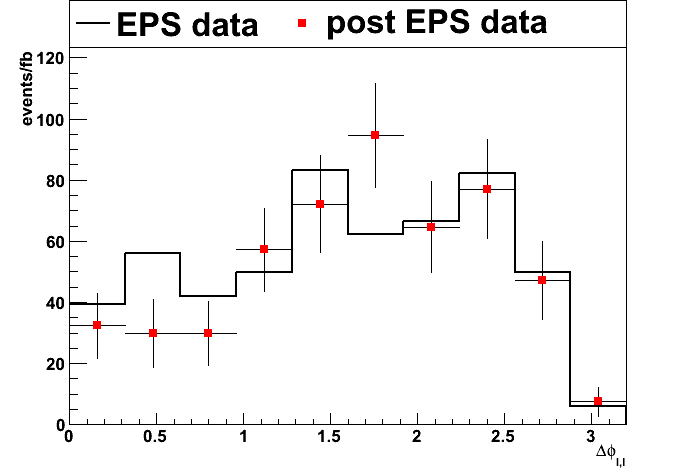
\includegraphics[width=.32\textwidth]{lp_figures/postEPSvalid/hm0/dPhi_ww0j.png}}
\subfigure[]{
\centering
\label{subfig:lp_dilepmass_ww0j}
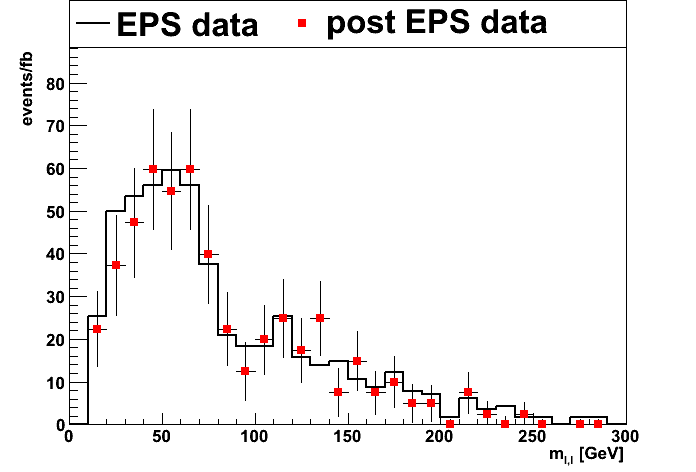
\includegraphics[width=.32\textwidth]{lp_figures/postEPSvalid/hm0/dilepmass_ww0j.png}}\\
\subfigure[]{
\centering
\label{subfig:lp_dileppt_ww0j}
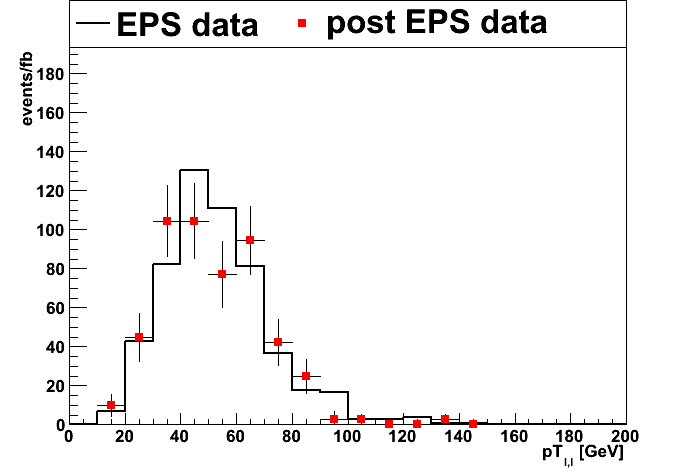
\includegraphics[width=.32\textwidth]{lp_figures/postEPSvalid/hm0/dileppt_ww0j.png}}
\subfigure[]{
\centering
\label{subfig:lp_type_ww0j}
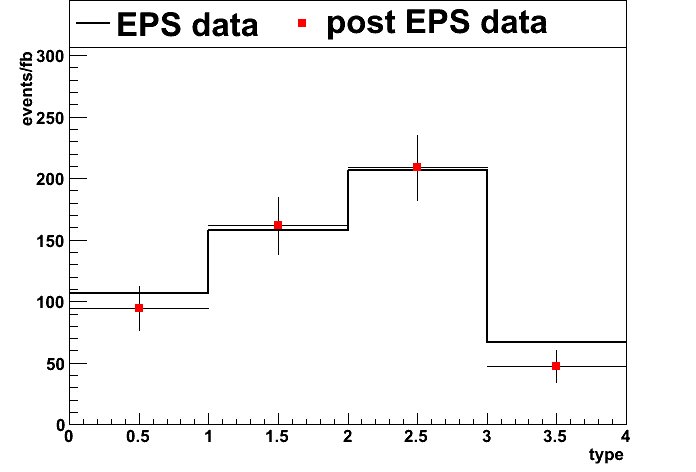
\includegraphics[width=.32\textwidth]{lp_figures/postEPSvalid/hm0/type_ww0j.png}}
\caption{EPS and post-EPS data comparison: 0-jet bin, all final states. 
\subref{subfig:lp_dPhi_ww0j} $\Delta\phi$ between the two leptons;
\subref{subfig:lp_dilepmass_ww0j} di-lepton invariant mass;
\subref{subfig:lp_dileppt_ww0j} di-lepton transverse momentum;
\subref{subfig:lp_type_ww0j} di-lepton type ($\mu\mu$=0, $\mu e$=2, $e\mu$=2, $ee$=3).
}
\label{fig:lp_ww0j_dilep}
\end{figure}

\begin{figure}[!hbtp]
\centering
\subfigure[]{
\centering
\label{subfig:lp_lep1pt_ww0j}
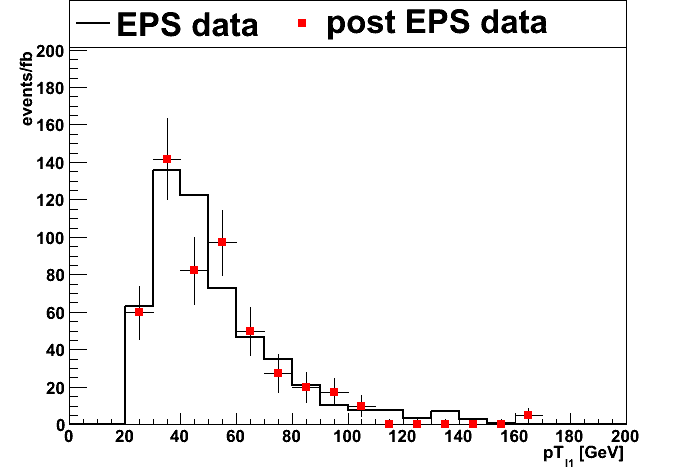
\includegraphics[width=.32\textwidth]{lp_figures/postEPSvalid/hm0/lep1pt_ww0j.png}}
\subfigure[]{
\centering
\label{subfig:lp_lep2pt_ww0j}
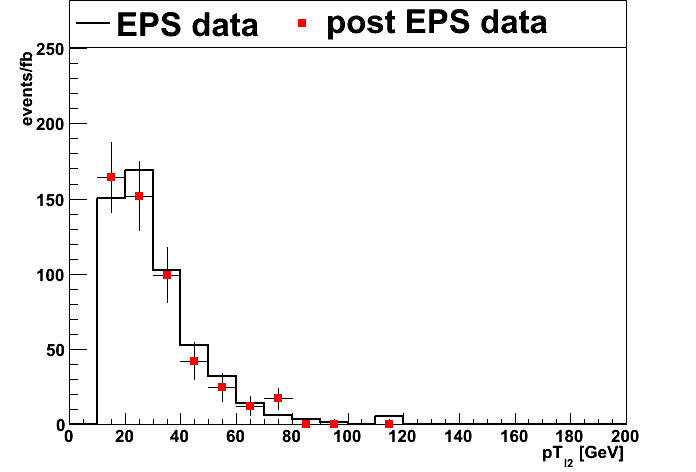
\includegraphics[width=.32\textwidth]{lp_figures/postEPSvalid/hm0/lep2pt_ww0j.png}}
\subfigure[]{
\centering
\label{subfig:lp_jet1pt_ww0j}
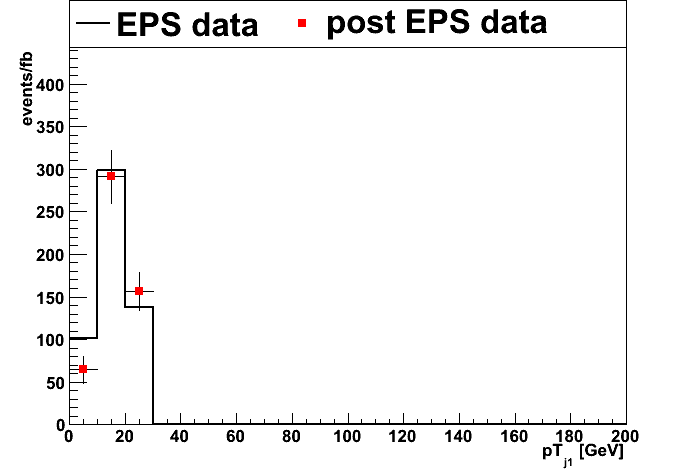
\includegraphics[width=.32\textwidth]{lp_figures/postEPSvalid/hm0/jet1pt_ww0j.png}}\\
\subfigure[]{
\centering
\label{subfig:lp_pmet_ww0j}
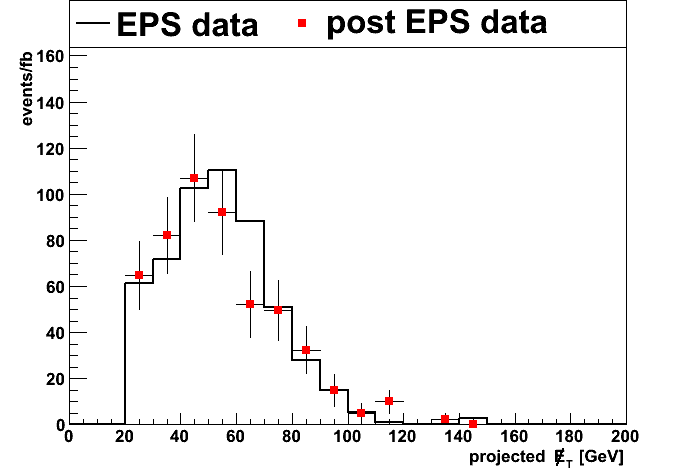
\includegraphics[width=.32\textwidth]{lp_figures/postEPSvalid/hm0/pmet_ww0j.png}}
\subfigure[]{
\centering
\label{subfig:lp_pTrackMet_ww0j}
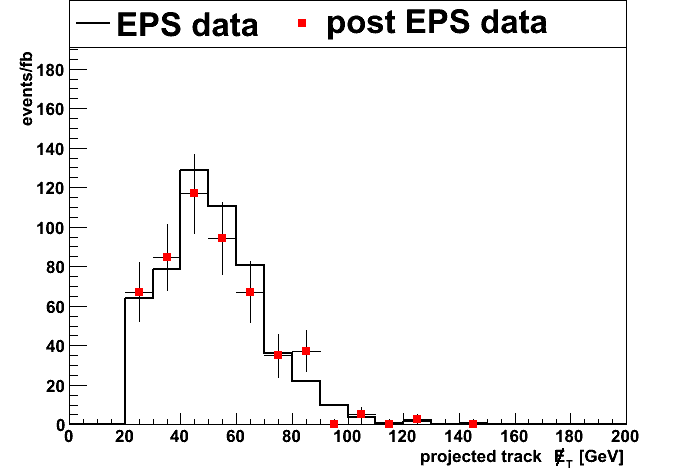
\includegraphics[width=.32\textwidth]{lp_figures/postEPSvalid/hm0/pTrackMet_ww0j.png}}
\subfigure[]{
\centering
\label{subfig:lp_mt_ww0j}
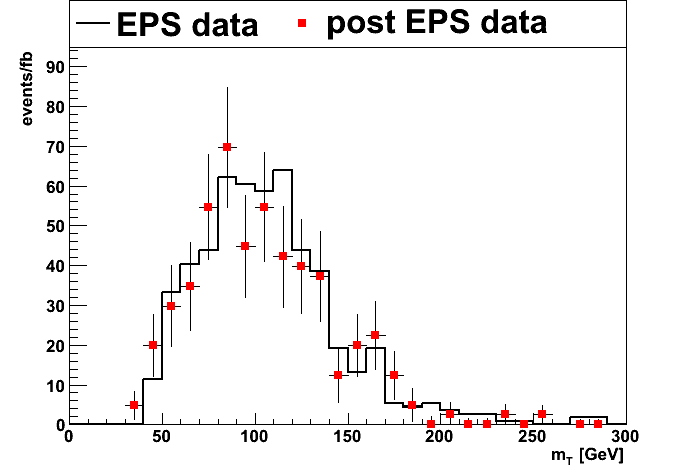
\includegraphics[width=.32\textwidth]{lp_figures/postEPSvalid/hm0/mt_ww0j.png}}
\caption{EPS and post-EPS data comparison: 0-jet bin, all final states. 
\subref{subfig:lp_lep1pt_ww0j} leading lepton $p_T$;
\subref{subfig:lp_lep2pt_ww0j} trailing lepton $p_T$;
\subref{subfig:lp_jet1pt_ww0j} leading jet $p_T$;
\subref{subfig:lp_pmet_ww0j} projected MET;
\subref{subfig:lp_pTrackMet_ww0j} projected track-MET;
\subref{subfig:lp_mt_ww0j} transverse mass of dilepton-MET system.
}
\label{fig:lp_ww0j_lepjetmet}
\end{figure}

\clearpage

\begin{figure}[!hbtp]
\centering
\subfigure[]{
\centering
\label{subfig:lp_dPhi_ww0jmm}
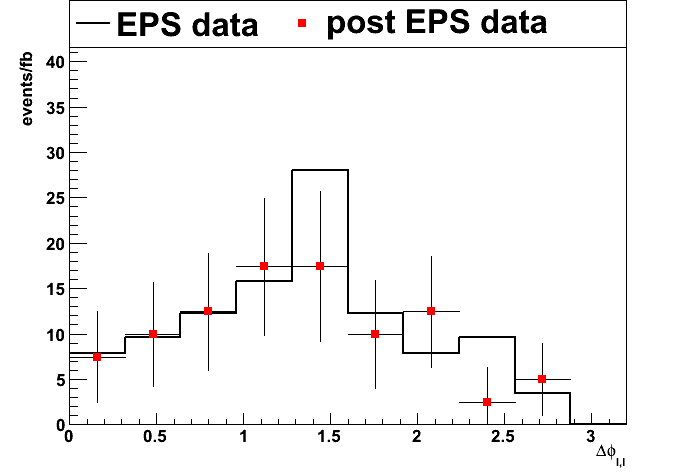
\includegraphics[width=.32\textwidth]{lp_figures/postEPSvalid/hm0/dPhi_ww0jmm.png}}
\subfigure[]{
\centering
\label{subfig:lp_dilepmass_ww0jmm}
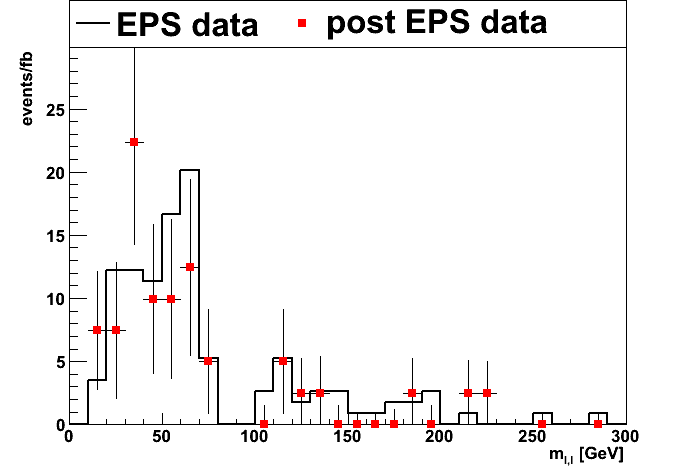
\includegraphics[width=.32\textwidth]{lp_figures/postEPSvalid/hm0/dilepmass_ww0jmm.png}}\\
\subfigure[]{
\centering
\label{subfig:lp_dileppt_ww0jmm}
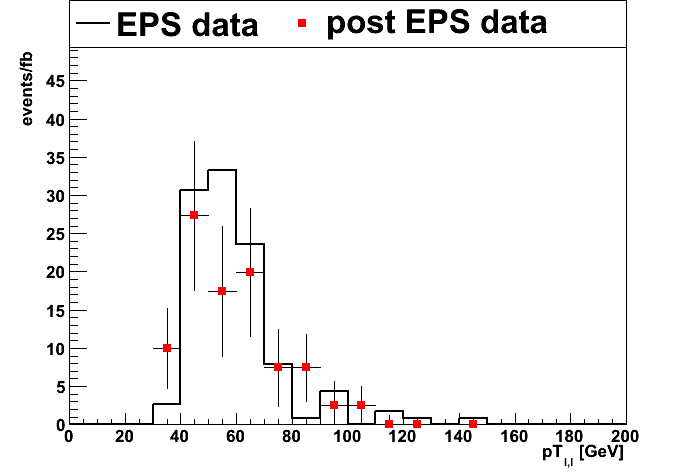
\includegraphics[width=.32\textwidth]{lp_figures/postEPSvalid/hm0/dileppt_ww0jmm.png}}
\subfigure[]{
\centering
\label{subfig:lp_type_ww0jmm}
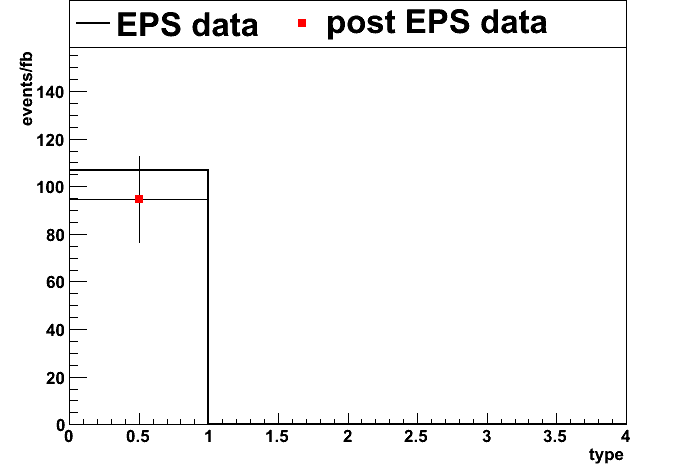
\includegraphics[width=.32\textwidth]{lp_figures/postEPSvalid/hm0/type_ww0jmm.png}}
\caption{EPS and post-EPS data comparison: 0-jet bin, $\mu\mu$ final state. 
\subref{subfig:lp_dPhi_ww0jmm} $\Delta\phi$ between the two leptons;
\subref{subfig:lp_dilepmass_ww0jmm} di-lepton invariant mass;
\subref{subfig:lp_dileppt_ww0jmm} di-lepton transverse momentum;
\subref{subfig:lp_type_ww0jmm} di-lepton type ($\mu\mu$=0, $\mu e$=2, $e\mu$=2, $ee$=3).
}
\label{fig:lp_ww0jmm_dilep}
\end{figure}

\begin{figure}[!hbtp]
\centering
\subfigure[]{
\centering
\label{subfig:lp_lep1pt_ww0jmm}
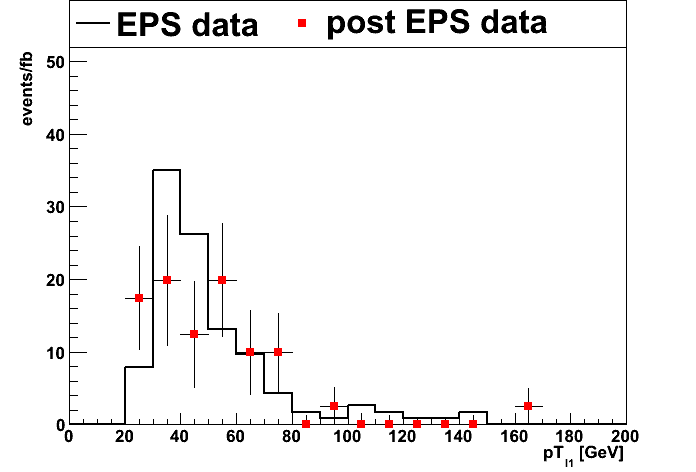
\includegraphics[width=.32\textwidth]{lp_figures/postEPSvalid/hm0/lep1pt_ww0jmm.png}}
\subfigure[]{
\centering
\label{subfig:lp_lep2pt_ww0jmm}
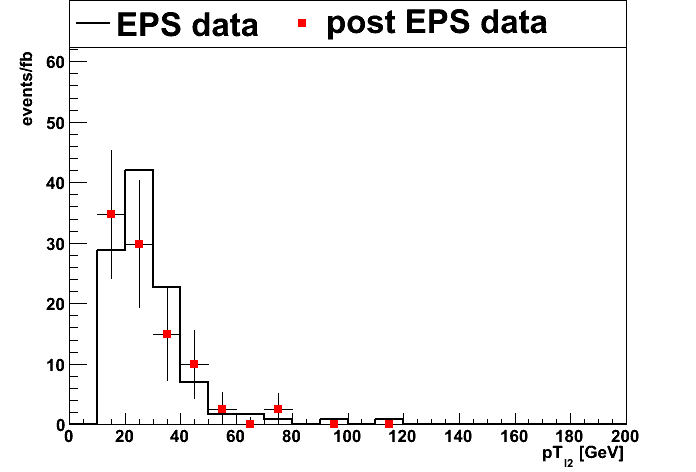
\includegraphics[width=.32\textwidth]{lp_figures/postEPSvalid/hm0/lep2pt_ww0jmm.png}}
\subfigure[]{
\centering
\label{subfig:lp_jet1pt_ww0jmm}
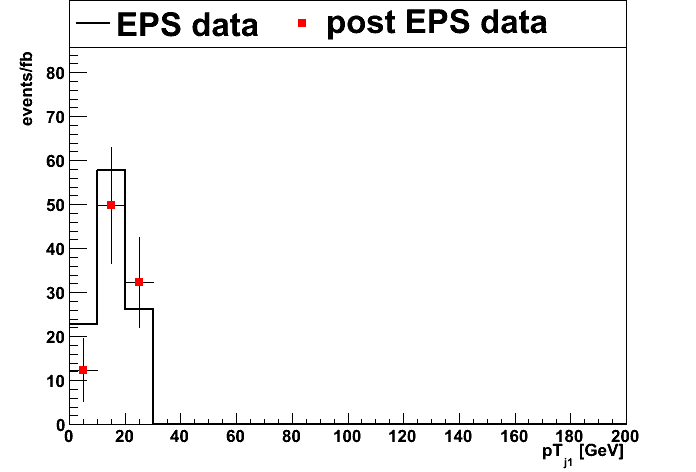
\includegraphics[width=.32\textwidth]{lp_figures/postEPSvalid/hm0/jet1pt_ww0jmm.png}}\\
\subfigure[]{
\centering
\label{subfig:lp_pmet_ww0jmm}
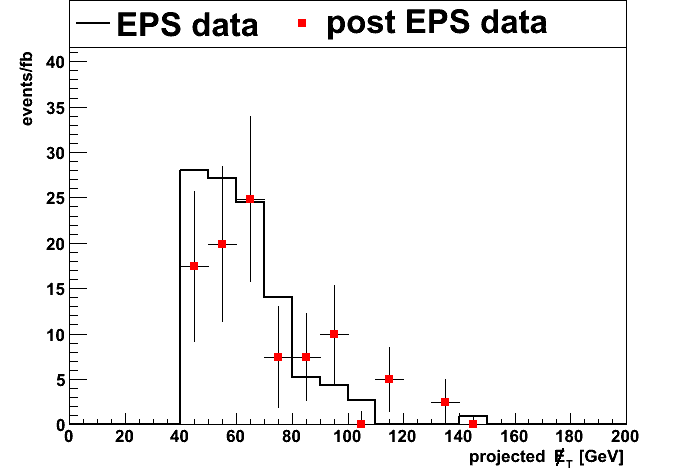
\includegraphics[width=.32\textwidth]{lp_figures/postEPSvalid/hm0/pmet_ww0jmm.png}}
\subfigure[]{
\centering
\label{subfig:lp_pTrackMet_ww0jmm}
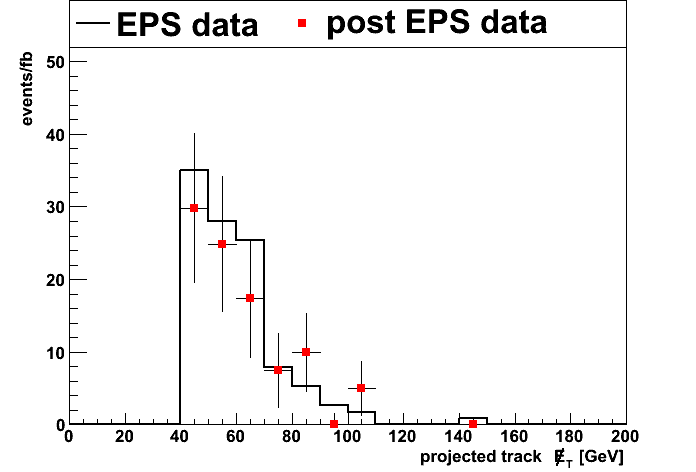
\includegraphics[width=.32\textwidth]{lp_figures/postEPSvalid/hm0/pTrackMet_ww0jmm.png}}
\subfigure[]{
\centering
\label{subfig:lp_mt_ww0jmm}
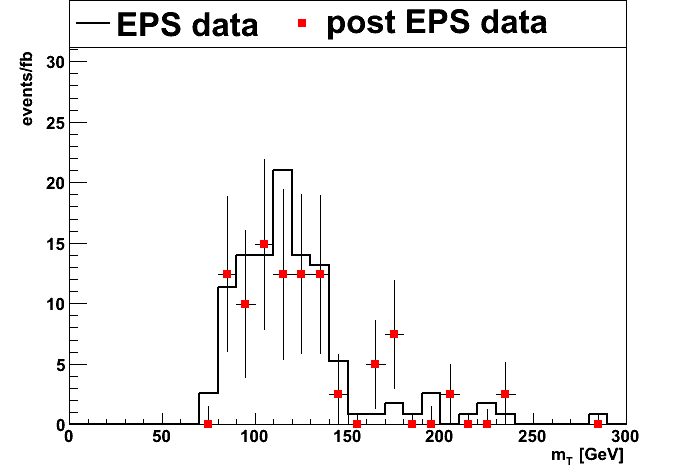
\includegraphics[width=.32\textwidth]{lp_figures/postEPSvalid/hm0/mt_ww0jmm.png}}
\caption{EPS and post-EPS data comparison: 0-jet bin, $\mu\mu$ final state. 
\subref{subfig:lp_lep1pt_ww0jmm} leading lepton $p_T$;
\subref{subfig:lp_lep2pt_ww0jmm} trailing lepton $p_T$;
\subref{subfig:lp_jet1pt_ww0jmm} leading jet $p_T$;
\subref{subfig:lp_pmet_ww0jmm} projected MET;
\subref{subfig:lp_pTrackMet_ww0jmm} projected track-MET;
\subref{subfig:lp_mt_ww0jmm} transverse mass of dilepton-MET system.
}
\label{fig:lp_ww0jmm_lepjetmet}
\end{figure}

\clearpage

\begin{figure}[!hbtp]
\centering
\subfigure[]{
\centering
\label{subfig:lp_dPhi_ww1j}
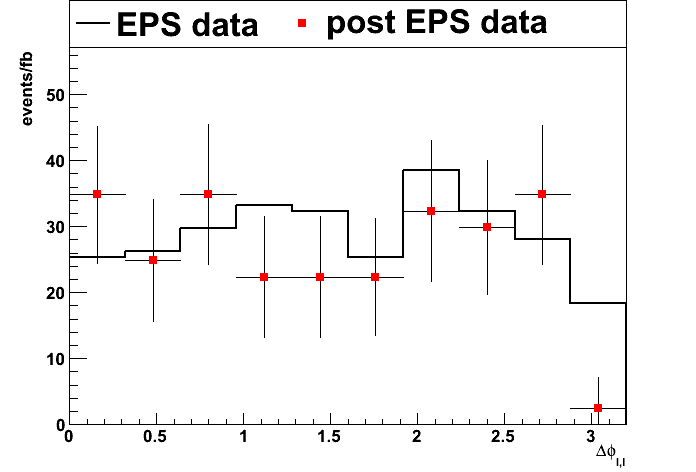
\includegraphics[width=.32\textwidth]{lp_figures/postEPSvalid/hm0/dPhi_ww1j.png}}
\subfigure[]{
\centering
\label{subfig:lp_dilepmass_ww1j}
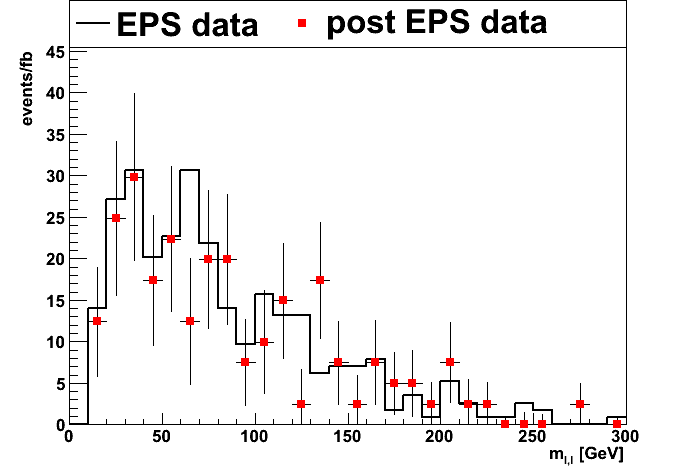
\includegraphics[width=.32\textwidth]{lp_figures/postEPSvalid/hm0/dilepmass_ww1j.png}}\\
\subfigure[]{
\centering
\label{subfig:lp_dileppt_ww1j}
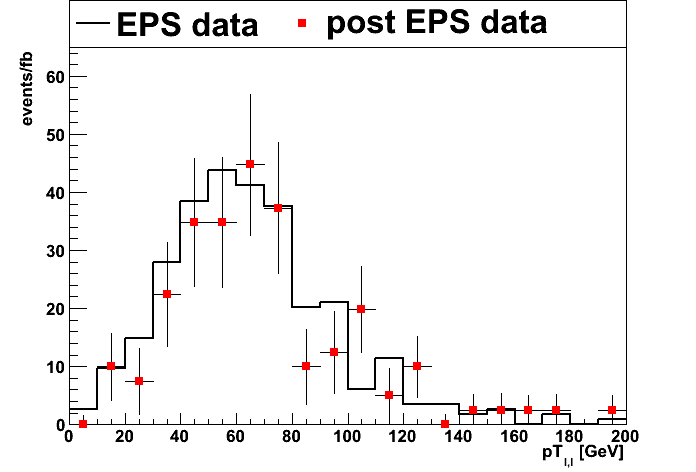
\includegraphics[width=.32\textwidth]{lp_figures/postEPSvalid/hm0/dileppt_ww1j.png}}
\subfigure[]{
\centering
\label{subfig:lp_type_ww1j}
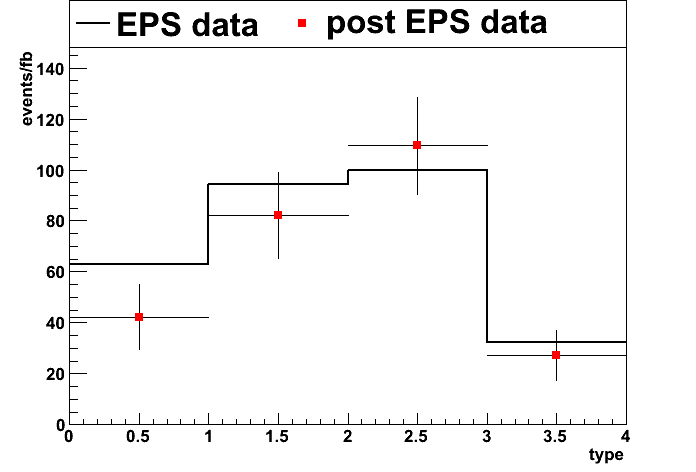
\includegraphics[width=.32\textwidth]{lp_figures/postEPSvalid/hm0/type_ww1j.png}}
\caption{EPS and post-EPS data comparison: 1-jet bin, all final states. 
\subref{subfig:lp_dPhi_ww1j} $\Delta\phi$ between the two leptons;
\subref{subfig:lp_dilepmass_ww1j} di-lepton invariant mass;
\subref{subfig:lp_dileppt_ww1j} di-lepton transverse momentum;
\subref{subfig:lp_type_ww1j} di-lepton type ($\mu\mu$=0, $\mu e$=2, $e\mu$=2, $ee$=3).
}
\label{fig:lp_ww1j_dilep}
\end{figure}

\begin{figure}[!hbtp]
\centering
\subfigure[]{
\centering
\label{subfig:lp_lep1pt_ww1j}
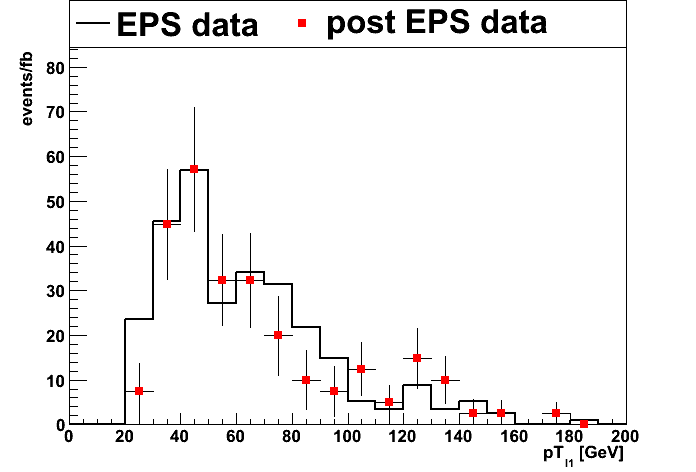
\includegraphics[width=.32\textwidth]{lp_figures/postEPSvalid/hm0/lep1pt_ww1j.png}}
\subfigure[]{
\centering
\label{subfig:lp_lep2pt_ww1j}
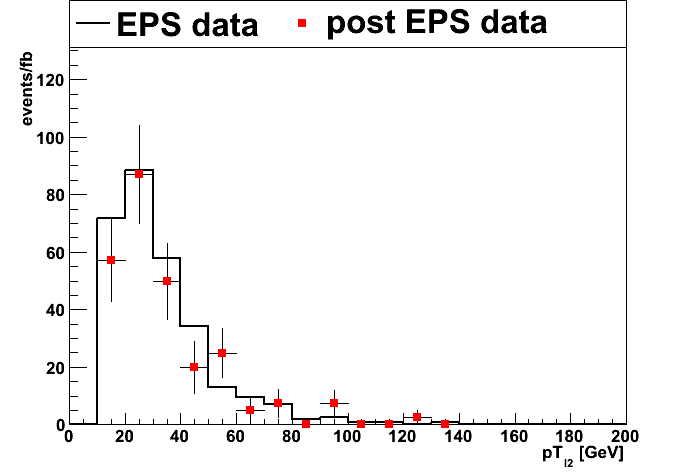
\includegraphics[width=.32\textwidth]{lp_figures/postEPSvalid/hm0/lep2pt_ww1j.png}}
\subfigure[]{
\centering
\label{subfig:lp_jet1pt_ww1j}
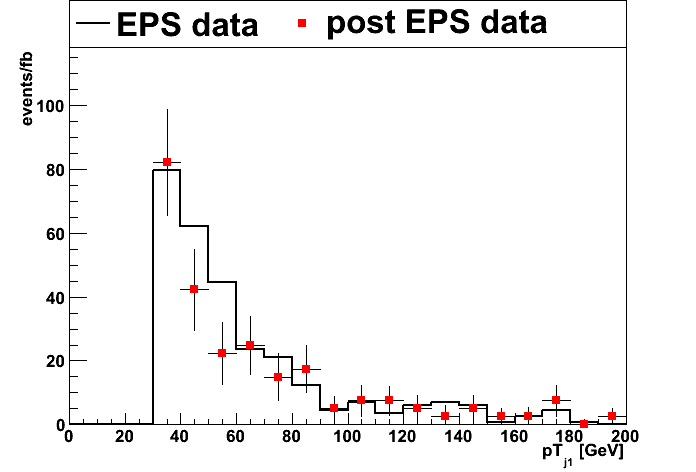
\includegraphics[width=.32\textwidth]{lp_figures/postEPSvalid/hm0/jet1pt_ww1j.png}}\\
\subfigure[]{
\centering
\label{subfig:lp_pmet_ww1j}
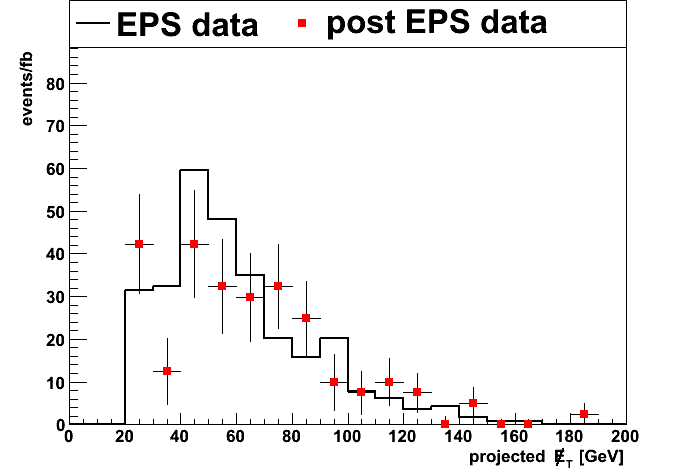
\includegraphics[width=.32\textwidth]{lp_figures/postEPSvalid/hm0/pmet_ww1j.png}}
\subfigure[]{
\centering
\label{subfig:lp_pTrackMet_ww1j}
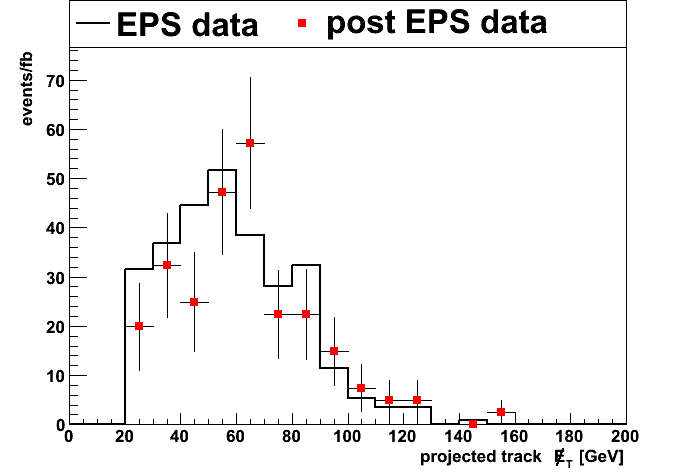
\includegraphics[width=.32\textwidth]{lp_figures/postEPSvalid/hm0/pTrackMet_ww1j.png}}
\subfigure[]{
\centering
\label{subfig:lp_mt_ww1j}
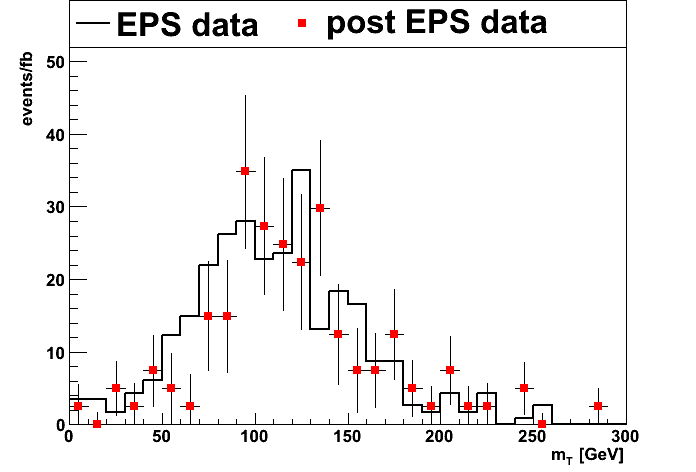
\includegraphics[width=.32\textwidth]{lp_figures/postEPSvalid/hm0/mt_ww1j.png}}
\caption{EPS and post-EPS data comparison: 1-jet bin, all final states. 
\subref{subfig:lp_lep1pt_ww1j} leading lepton $p_T$;
\subref{subfig:lp_lep2pt_ww1j} trailing lepton $p_T$;
\subref{subfig:lp_jet1pt_ww1j} leading jet $p_T$;
\subref{subfig:lp_pmet_ww1j} projected MET;
\subref{subfig:lp_pTrackMet_ww1j} projected track-MET;
\subref{subfig:lp_mt_ww1j} transverse mass of dilepton-MET system.
}
\label{fig:lp_ww1j_lepjetmet}
\end{figure}

\clearpage

\begin{figure}[!hbtp]
\centering
\subfigure[]{
\centering
\label{subfig:lp_dPhi_ww2j}
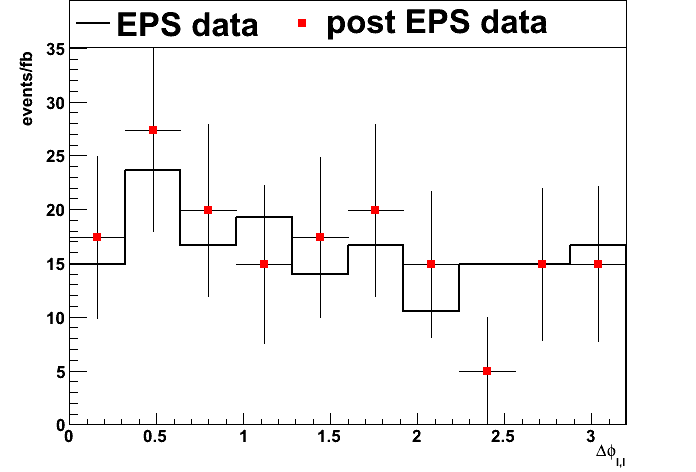
\includegraphics[width=.32\textwidth]{lp_figures/postEPSvalid/hm0/dPhi_ww2j.png}}
\subfigure[]{
\centering
\label{subfig:lp_dilepmass_ww2j}
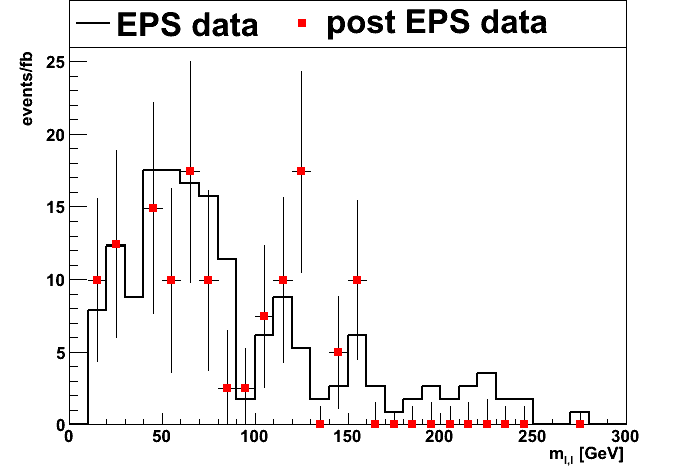
\includegraphics[width=.32\textwidth]{lp_figures/postEPSvalid/hm0/dilepmass_ww2j.png}}\\
\subfigure[]{
\centering
\label{subfig:lp_dileppt_ww2j}
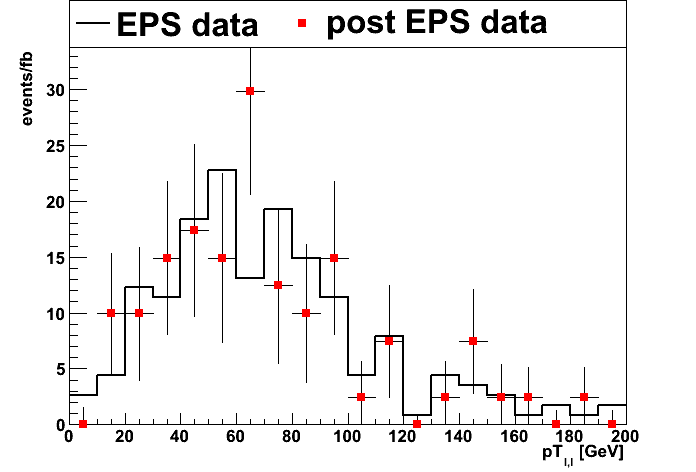
\includegraphics[width=.32\textwidth]{lp_figures/postEPSvalid/hm0/dileppt_ww2j.png}}
\subfigure[]{
\centering
\label{subfig:lp_type_ww2j}
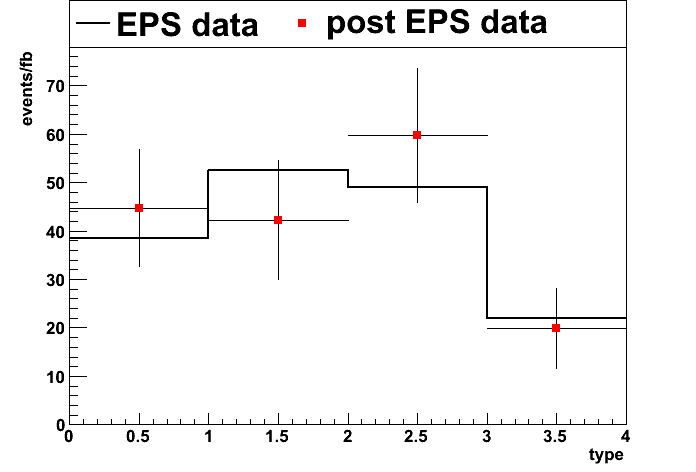
\includegraphics[width=.32\textwidth]{lp_figures/postEPSvalid/hm0/type_ww2j.png}}
\caption{EPS and post-EPS data comparison: 2-jet bin, all final states. 
\subref{subfig:lp_dPhi_ww2j} $\Delta\phi$ between the two leptons;
\subref{subfig:lp_dilepmass_ww2j} di-lepton invariant mass;
\subref{subfig:lp_dileppt_ww2j} di-lepton transverse momentum;
\subref{subfig:lp_type_ww2j} di-lepton type ($\mu\mu$=0, $\mu e$=2, $e\mu$=2, $ee$=3).
}
\label{fig:lp_ww2j_dilep}
\end{figure}

\begin{figure}[!hbtp]
\centering
\subfigure[]{
\centering
\label{subfig:lp_lep1pt_ww2j}
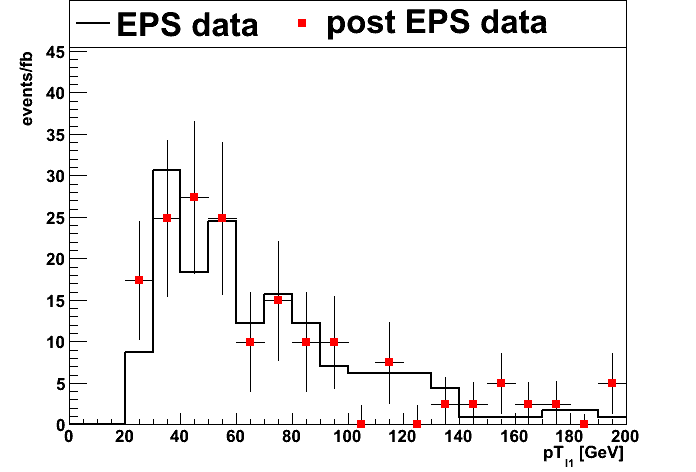
\includegraphics[width=.32\textwidth]{lp_figures/postEPSvalid/hm0/lep1pt_ww2j.png}}
\subfigure[]{
\centering
\label{subfig:lp_lep2pt_ww2j}
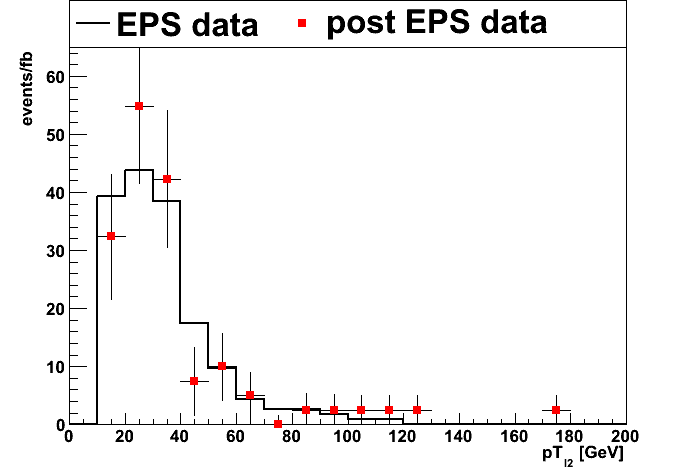
\includegraphics[width=.32\textwidth]{lp_figures/postEPSvalid/hm0/lep2pt_ww2j.png}}
\subfigure[]{
\centering
\label{subfig:lp_jet1pt_ww2j}
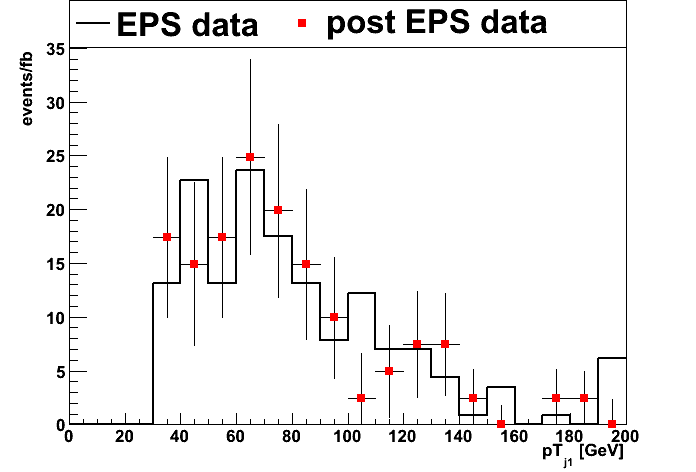
\includegraphics[width=.32\textwidth]{lp_figures/postEPSvalid/hm0/jet1pt_ww2j.png}}\\
\subfigure[]{
\centering
\label{subfig:lp_pmet_ww2j}
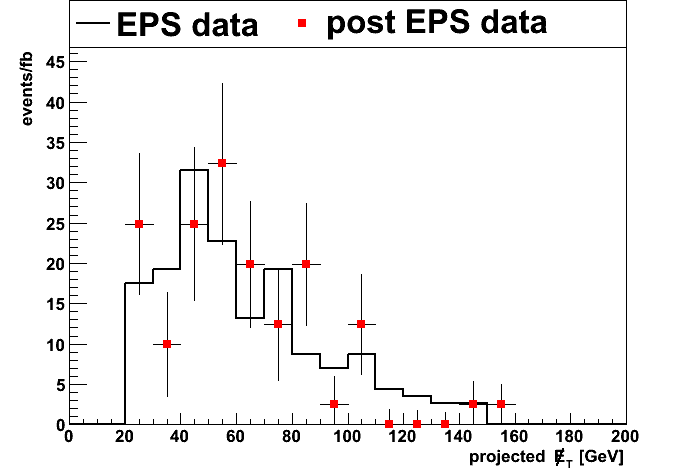
\includegraphics[width=.32\textwidth]{lp_figures/postEPSvalid/hm0/pmet_ww2j.png}}
\subfigure[]{
\centering
\label{subfig:lp_pTrackMet_ww2j}
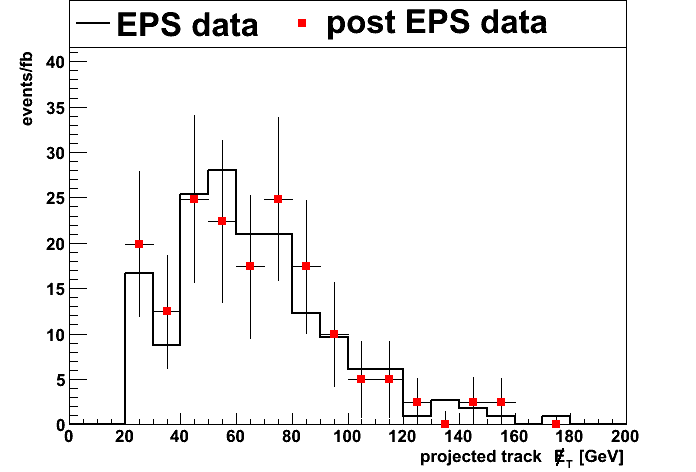
\includegraphics[width=.32\textwidth]{lp_figures/postEPSvalid/hm0/pTrackMet_ww2j.png}}
\subfigure[]{
\centering
\label{subfig:lp_mt_ww2j}
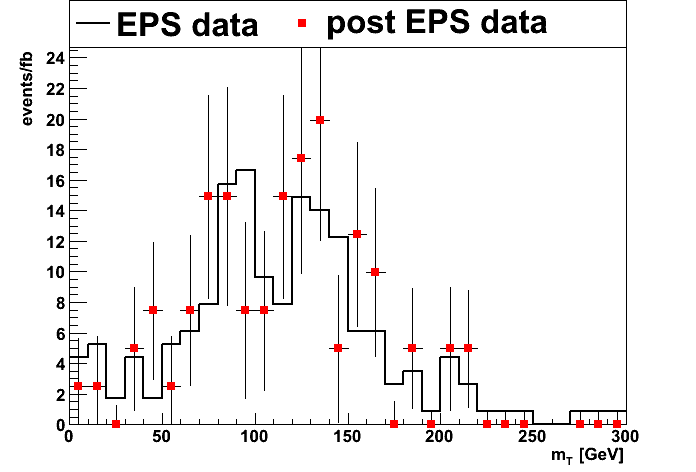
\includegraphics[width=.32\textwidth]{lp_figures/postEPSvalid/hm0/mt_ww2j.png}}
\caption{EPS and post-EPS data comparison: 2-jet bin, all final states. 
\subref{subfig:lp_lep1pt_ww2j} leading lepton $p_T$;
\subref{subfig:lp_lep2pt_ww2j} trailing lepton $p_T$;
\subref{subfig:lp_jet1pt_ww2j} leading jet $p_T$;
\subref{subfig:lp_pmet_ww2j} projected MET;
\subref{subfig:lp_pTrackMet_ww2j} projected track-MET;
\subref{subfig:lp_mt_ww2j} transverse mass of dilepton-MET system.
}
\label{fig:lp_ww2j_lepjetmet}
\end{figure}

\clearpage

\subsubsection{Data to Simulation Distributions}

In this section, the data validation is performed by comparing the data in each dataset (EPS, post-EPS, LP) with MC prediction scaled to 
data-driven estimations.

Six distributions are shown in Figures~\ref{fig:ww_deltaphi_lp}-\ref{fig:ww_ptmin_lp}: $\Delta\phi$, dilepton mass, transverse mass, 
min-MET, leading and trailing lepton $p_T$. Each figure contains plots for EPS, post-EPS, LP data in the 0-, 1- and 2-jet bins.

The agreement between data in the different data samples with MC is very good.

\begin{figure}[!hbtp]
\centering
\subfigure[]{
\centering
\label{subfig:ww_deltaphi_0j_EPS}
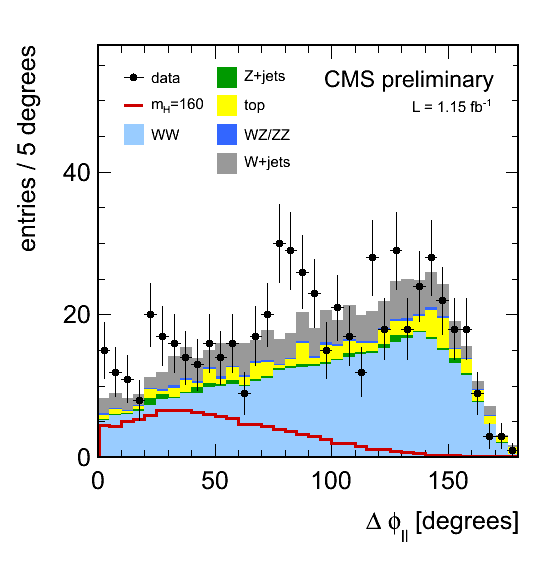
\includegraphics[width=.32\textwidth]{lp_figures/histo_deltaphill_ww0j_allhwwcuts_EPS.png}}
\subfigure[]{
\centering
\label{subfig:ww_deltaphi_1j_EPS}
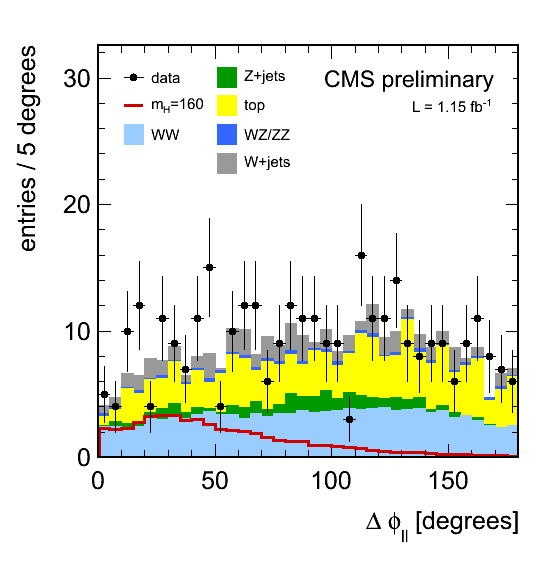
\includegraphics[width=.32\textwidth]{lp_figures/histo_deltaphill_ww1j_allhwwcuts_EPS.png}}
\subfigure[]{
\centering
\label{subfig:ww_deltaphi_2j_EPS}
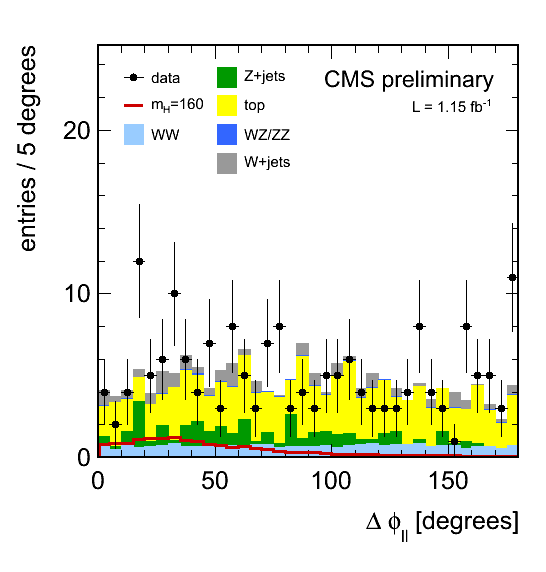
\includegraphics[width=.32\textwidth]{lp_figures/histo_deltaphill_ww2j_allhwwcuts_EPS.png}}\\
\subfigure[]{
\centering
\label{subfig:ww_deltaphi_0j_POSTEPS}
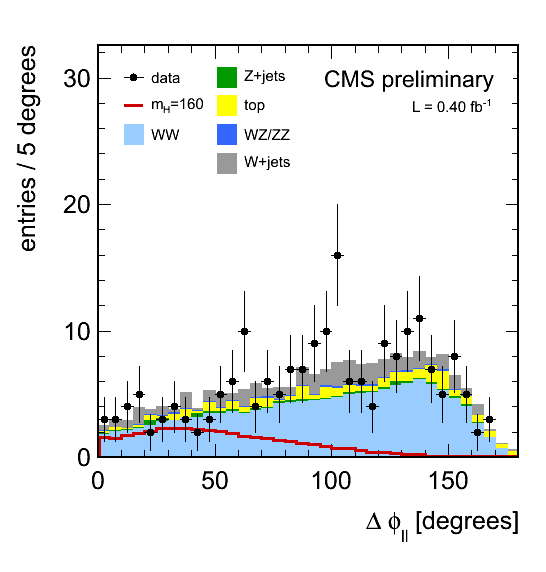
\includegraphics[width=.32\textwidth]{lp_figures/histo_deltaphill_ww0j_allhwwcuts_POSTEPS.png}}
\subfigure[]{
\centering
\label{subfig:ww_deltaphi_1j_POSTEPS}
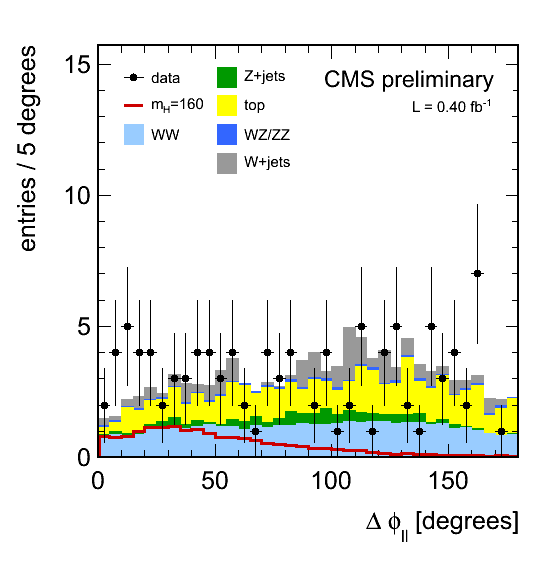
\includegraphics[width=.32\textwidth]{lp_figures/histo_deltaphill_ww1j_allhwwcuts_POSTEPS.png}}
\subfigure[]{
\centering
\label{subfig:ww_deltaphi_2j_POSTEPS}
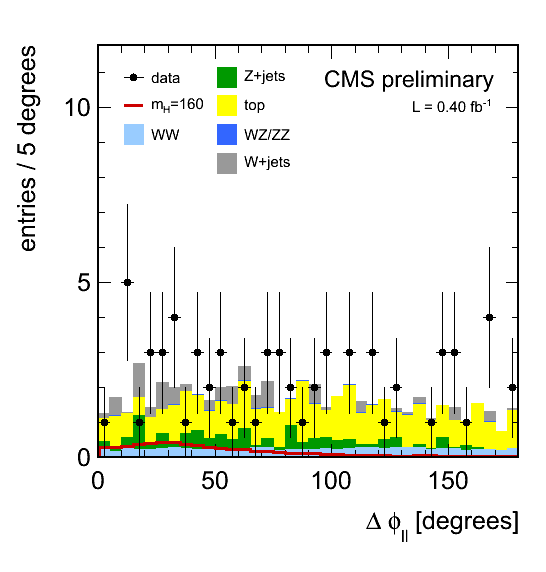
\includegraphics[width=.32\textwidth]{lp_figures/histo_deltaphill_ww2j_allhwwcuts_POSTEPS.png}}\\
\subfigure[]{
\centering
\label{subfig:ww_deltaphi_0j_LP}
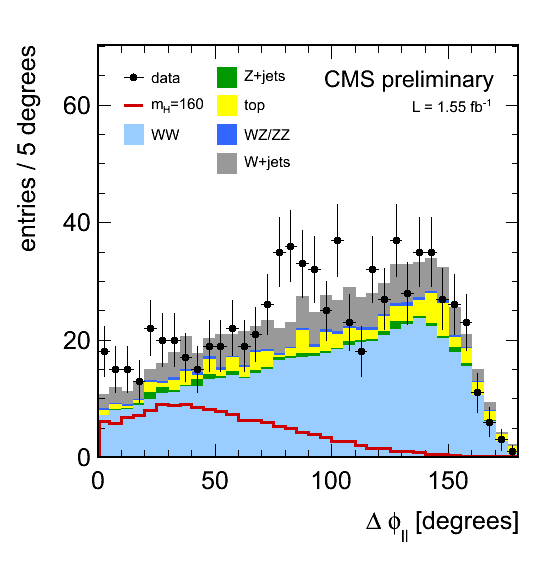
\includegraphics[width=.32\textwidth]{lp_figures/histo_deltaphill_ww0j_allhwwcuts.png}}
\subfigure[]{
\centering
\label{subfig:ww_deltaphi_1j_LP}
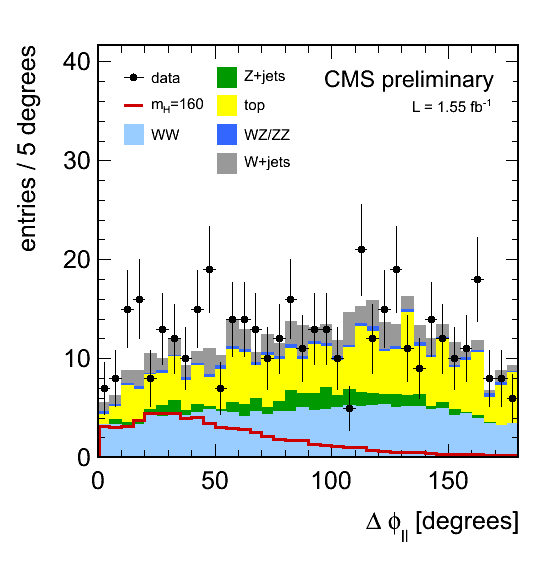
\includegraphics[width=.32\textwidth]{lp_figures/histo_deltaphill_ww1j_allhwwcuts.png}}
\subfigure[]{
\centering
\label{subfig:ww_deltaphi_2j_LP}
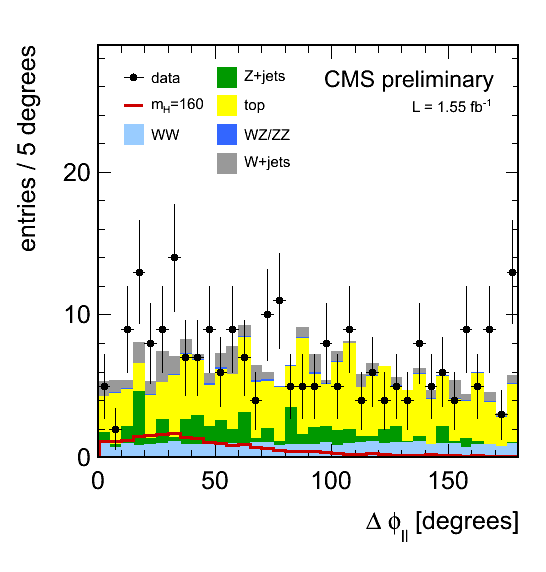
\includegraphics[width=.32\textwidth]{lp_figures/histo_deltaphill_ww2j_allhwwcuts.png}}\\
\caption{
Dilepton $\Delta\phi$ distribution after WW selection for \lpintlumi of data in the 0-jet (left), 
1-jet (middle) and 2-jet (right) bin analyses in the EPS (top), post-EPS (center) and LP (bottom) datasets.
MC is scaled to data-driven estimates.
}
\label{fig:ww_deltaphi_lp}
\end{figure}

\clearpage

\begin{figure}[!hbtp]
\centering
\subfigure[]{
\centering
\label{subfig:ww_mass_0j_EPS}
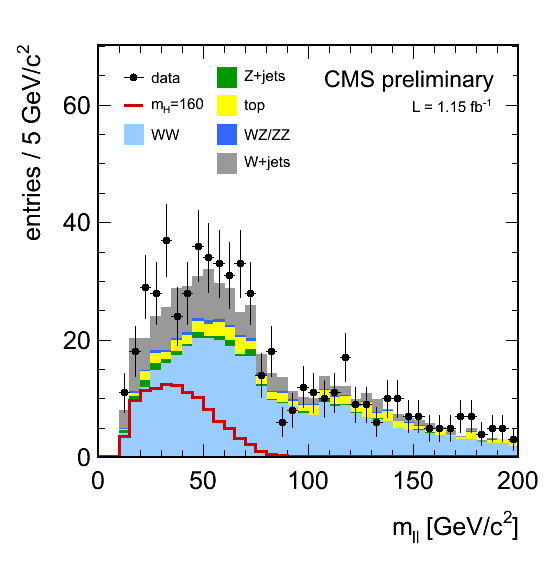
\includegraphics[width=.32\textwidth]{lp_figures/histo_massll_ww0j_allhwwcuts_EPS.png}}
\subfigure[]{
\centering
\label{subfig:ww_mass_1j_EPS}
\includegraphics[width=.32\textwidth]{lp_figures/histo_massll_ww1j_allhwwcuts_EPS.png}}
\subfigure[]{
\centering
\label{subfig:ww_mass_2j_EPS}
\includegraphics[width=.32\textwidth]{lp_figures/histo_massll_ww2j_allhwwcuts_EPS.png}}\\
\subfigure[]{
\centering
\label{subfig:ww_mass_0j_POSTEPS}
\includegraphics[width=.32\textwidth]{lp_figures/histo_massll_ww0j_allhwwcuts_POSTEPS.png}}
\subfigure[]{
\centering
\label{subfig:ww_mass_1j_POSTEPS}
\includegraphics[width=.32\textwidth]{lp_figures/histo_massll_ww1j_allhwwcuts_POSTEPS.png}}
\subfigure[]{
\centering
\label{subfig:ww_mass_2j_POSTEPS}
\includegraphics[width=.32\textwidth]{lp_figures/histo_massll_ww2j_allhwwcuts_POSTEPS.png}}\\
\subfigure[]{
\centering
\label{subfig:ww_mass_0j_LP}
\includegraphics[width=.32\textwidth]{lp_figures/histo_massll_ww0j_allhwwcuts.png}}
\subfigure[]{
\centering
\label{subfig:ww_mass_1j_LP}
\includegraphics[width=.32\textwidth]{lp_figures/histo_massll_ww1j_allhwwcuts.png}}
\subfigure[]{
\centering
\label{subfig:ww_mass_2j_LP}
\includegraphics[width=.32\textwidth]{lp_figures/histo_massll_ww2j_allhwwcuts.png}}\\
\caption{
Dilepton invariant mass distribution after WW selection for \lpintlumi of data in the 0-jet (left), 
1-jet (middle) and 2-jet (right) bin analyses in the EPS (top), post-EPS (center) and LP (bottom) datasets.
MC is scaled to data-driven estimates.
}
\label{fig:ww_mass_lp}
\end{figure}

\clearpage

\begin{figure}[!hbtp]
\centering
\subfigure[]{
\centering
\label{subfig:ww_mthiggs_0j_EPS}
\includegraphics[width=.32\textwidth]{lp_figures/histo_mthiggs_ww0j_allhwwcuts_EPS.png}}
\subfigure[]{
\centering
\label{subfig:ww_mthiggs_1j_EPS}
\includegraphics[width=.32\textwidth]{lp_figures/histo_mthiggs_ww1j_allhwwcuts_EPS.png}}
\subfigure[]{
\centering
\label{subfig:ww_mthiggs_2j_EPS}
\includegraphics[width=.32\textwidth]{lp_figures/histo_mthiggs_ww2j_allhwwcuts_EPS.png}}\\
\subfigure[]{
\centering
\label{subfig:ww_mthiggs_0j_POSTEPS}
\includegraphics[width=.32\textwidth]{lp_figures/histo_mthiggs_ww0j_allhwwcuts_POSTEPS.png}}
\subfigure[]{
\centering
\label{subfig:ww_mthiggs_1j_POSTEPS}
\includegraphics[width=.32\textwidth]{lp_figures/histo_mthiggs_ww1j_allhwwcuts_POSTEPS.png}}
\subfigure[]{
\centering
\label{subfig:ww_mthiggs_2j_POSTEPS}
\includegraphics[width=.32\textwidth]{lp_figures/histo_mthiggs_ww2j_allhwwcuts_POSTEPS.png}}\\
\subfigure[]{
\centering
\label{subfig:ww_mthiggs_0j_LP}
\includegraphics[width=.32\textwidth]{lp_figures/histo_mthiggs_ww0j_allhwwcuts.png}}
\subfigure[]{
\centering
\label{subfig:ww_mthiggs_1j_LP}
\includegraphics[width=.32\textwidth]{lp_figures/histo_mthiggs_ww1j_allhwwcuts.png}}
\subfigure[]{
\centering
\label{subfig:ww_mthiggs_2j_LP}
\includegraphics[width=.32\textwidth]{lp_figures/histo_mthiggs_ww2j_allhwwcuts.png}}\\
\caption{
Dilepton-MET transverse mass distribution after WW selection for \lpintlumi of data in the 0-jet (left), 
1-jet (middle) and 2-jet (right) bin analyses in the EPS (top), post-EPS (center) and LP (bottom) datasets.
MC is scaled to data-driven estimates.
}
\label{fig:ww_mthiggs_lp}
\end{figure}

\clearpage

\begin{figure}[!hbtp]
\centering
\subfigure[]{
\centering
\label{subfig:ww_minpmet_0j_EPS}
\includegraphics[width=.32\textwidth]{lp_figures/histo_minpmet_ww0j_allhwwcuts_EPS.png}}
\subfigure[]{
\centering
\label{subfig:ww_minpmet_1j_EPS}
\includegraphics[width=.32\textwidth]{lp_figures/histo_minpmet_ww1j_allhwwcuts_EPS.png}}
\subfigure[]{
\centering
\label{subfig:ww_minpmet_2j_EPS}
\includegraphics[width=.32\textwidth]{lp_figures/histo_minpmet_ww2j_allhwwcuts_EPS.png}}\\
\subfigure[]{
\centering
\label{subfig:ww_minpmet_0j_POSTEPS}
\includegraphics[width=.32\textwidth]{lp_figures/histo_minpmet_ww0j_allhwwcuts_POSTEPS.png}}
\subfigure[]{
\centering
\label{subfig:ww_minpmet_1j_POSTEPS}
\includegraphics[width=.32\textwidth]{lp_figures/histo_minpmet_ww1j_allhwwcuts_POSTEPS.png}}
\subfigure[]{
\centering
\label{subfig:ww_minpmet_2j_POSTEPS}
\includegraphics[width=.32\textwidth]{lp_figures/histo_minpmet_ww2j_allhwwcuts_POSTEPS.png}}\\
\subfigure[]{
\centering
\label{subfig:ww_minpmet_0j_LP}
\includegraphics[width=.32\textwidth]{lp_figures/histo_minpmet_ww0j_allhwwcuts.png}}
\subfigure[]{
\centering
\label{subfig:ww_minpmet_1j_LP}
\includegraphics[width=.32\textwidth]{lp_figures/histo_minpmet_ww1j_allhwwcuts.png}}
\subfigure[]{
\centering
\label{subfig:ww_minpmet_2j_LP}
\includegraphics[width=.32\textwidth]{lp_figures/histo_minpmet_ww2j_allhwwcuts.png}}\\
\caption{
min-MET distribution after WW selection for \lpintlumi of data in the 0-jet (left), 
1-jet (middle) and 2-jet (right) bin analyses in the EPS (top), post-EPS (center) and LP (bottom) datasets.
MC is scaled to data-driven estimates.
}
\label{fig:ww_minpmet_lp}
\end{figure}

\clearpage

\begin{figure}[!hbtp]
\centering
\subfigure[]{
\centering
\label{subfig:ww_ptmax_0j_EPS}
\includegraphics[width=.32\textwidth]{lp_figures/histo_ptmax_ww0j_allhwwcuts_EPS.png}}
\subfigure[]{
\centering
\label{subfig:ww_ptmax_1j_EPS}
\includegraphics[width=.32\textwidth]{lp_figures/histo_ptmax_ww1j_allhwwcuts_EPS.png}}
\subfigure[]{
\centering
\label{subfig:ww_ptmax_2j_EPS}
\includegraphics[width=.32\textwidth]{lp_figures/histo_ptmax_ww2j_allhwwcuts_EPS.png}}\\
\subfigure[]{
\centering
\label{subfig:ww_ptmax_0j_POSTEPS}
\includegraphics[width=.32\textwidth]{lp_figures/histo_ptmax_ww0j_allhwwcuts_POSTEPS.png}}
\subfigure[]{
\centering
\label{subfig:ww_ptmax_1j_POSTEPS}
\includegraphics[width=.32\textwidth]{lp_figures/histo_ptmax_ww1j_allhwwcuts_POSTEPS.png}}
\subfigure[]{
\centering
\label{subfig:ww_ptmax_2j_POSTEPS}
\includegraphics[width=.32\textwidth]{lp_figures/histo_ptmax_ww2j_allhwwcuts_POSTEPS.png}}\\
\subfigure[]{
\centering
\label{subfig:ww_ptmax_0j_LP}
\includegraphics[width=.32\textwidth]{lp_figures/histo_ptmax_ww0j_allhwwcuts.png}}
\subfigure[]{
\centering
\label{subfig:ww_ptmax_1j_LP}
\includegraphics[width=.32\textwidth]{lp_figures/histo_ptmax_ww1j_allhwwcuts.png}}
\subfigure[]{
\centering
\label{subfig:ww_ptmax_2j_LP}
\includegraphics[width=.32\textwidth]{lp_figures/histo_ptmax_ww2j_allhwwcuts.png}}\\
\caption{
Leading lepton $p_T$ distribution after WW selection for \lpintlumi of data in the 0-jet (left), 
1-jet (middle) and 2-jet (right) bin analyses in the EPS (top), post-EPS (center) and LP (bottom) datasets.
MC is scaled to data-driven estimates.
}
\label{fig:ww_ptmax_lp}
\end{figure}

\clearpage

\begin{figure}[!hbtp]
\centering
\subfigure[]{
\centering
\label{subfig:ww_ptmin_0j_EPS}
\includegraphics[width=.32\textwidth]{lp_figures/histo_ptmin_ww0j_allhwwcuts_EPS.png}}
\subfigure[]{
\centering
\label{subfig:ww_ptmin_1j_EPS}
\includegraphics[width=.32\textwidth]{lp_figures/histo_ptmin_ww1j_allhwwcuts_EPS.png}}
\subfigure[]{
\centering
\label{subfig:ww_ptmin_2j_EPS}
\includegraphics[width=.32\textwidth]{lp_figures/histo_ptmin_ww2j_allhwwcuts_EPS.png}}\\
\subfigure[]{
\centering
\label{subfig:ww_ptmin_0j_POSTEPS}
\includegraphics[width=.32\textwidth]{lp_figures/histo_ptmin_ww0j_allhwwcuts_POSTEPS.png}}
\subfigure[]{
\centering
\label{subfig:ww_ptmin_1j_POSTEPS}
\includegraphics[width=.32\textwidth]{lp_figures/histo_ptmin_ww1j_allhwwcuts_POSTEPS.png}}
\subfigure[]{
\centering
\label{subfig:ww_ptmin_2j_POSTEPS}
\includegraphics[width=.32\textwidth]{lp_figures/histo_ptmin_ww2j_allhwwcuts_POSTEPS.png}}\\
\subfigure[]{
\centering
\label{subfig:ww_ptmin_0j_LP}
\includegraphics[width=.32\textwidth]{lp_figures/histo_ptmin_ww0j_allhwwcuts.png}}
\subfigure[]{
\centering
\label{subfig:ww_ptmin_1j_LP}
\includegraphics[width=.32\textwidth]{lp_figures/histo_ptmin_ww1j_allhwwcuts.png}}
\subfigure[]{
\centering
\label{subfig:ww_ptmin_2j_LP}
\includegraphics[width=.32\textwidth]{lp_figures/histo_ptmin_ww2j_allhwwcuts.png}}\\
\caption{
Trailing lepton $p_T$ distribution after WW selection for \lpintlumi of data in the 0-jet (left), 
1-jet (middle) and 2-jet (right) bin analyses in the EPS (top), post-EPS (center) and LP (bottom) datasets.
MC is scaled to data-driven estimates.
}
\label{fig:ww_ptmin_lp}
\end{figure}

\clearpage
